% Wide, two-column-spanning figure (7 panels). Requires \usepackage{graphicx} and \usepackage{booktabs}.
% Put uncertainty_method_cmp_simpleqa.pdf on the graphics path (\graphicspath{{figures/}}) or use a full path.
% Citation keys li2023iti / selfaware / falseqa / simpleqa are defined in docs/blade-method.bib.
% This EXTENDS fig_uncertainty_method_cmp.tex with two SimpleQA panels; it is a separate figure/file.
\begin{figure*}[t]
  \centering
  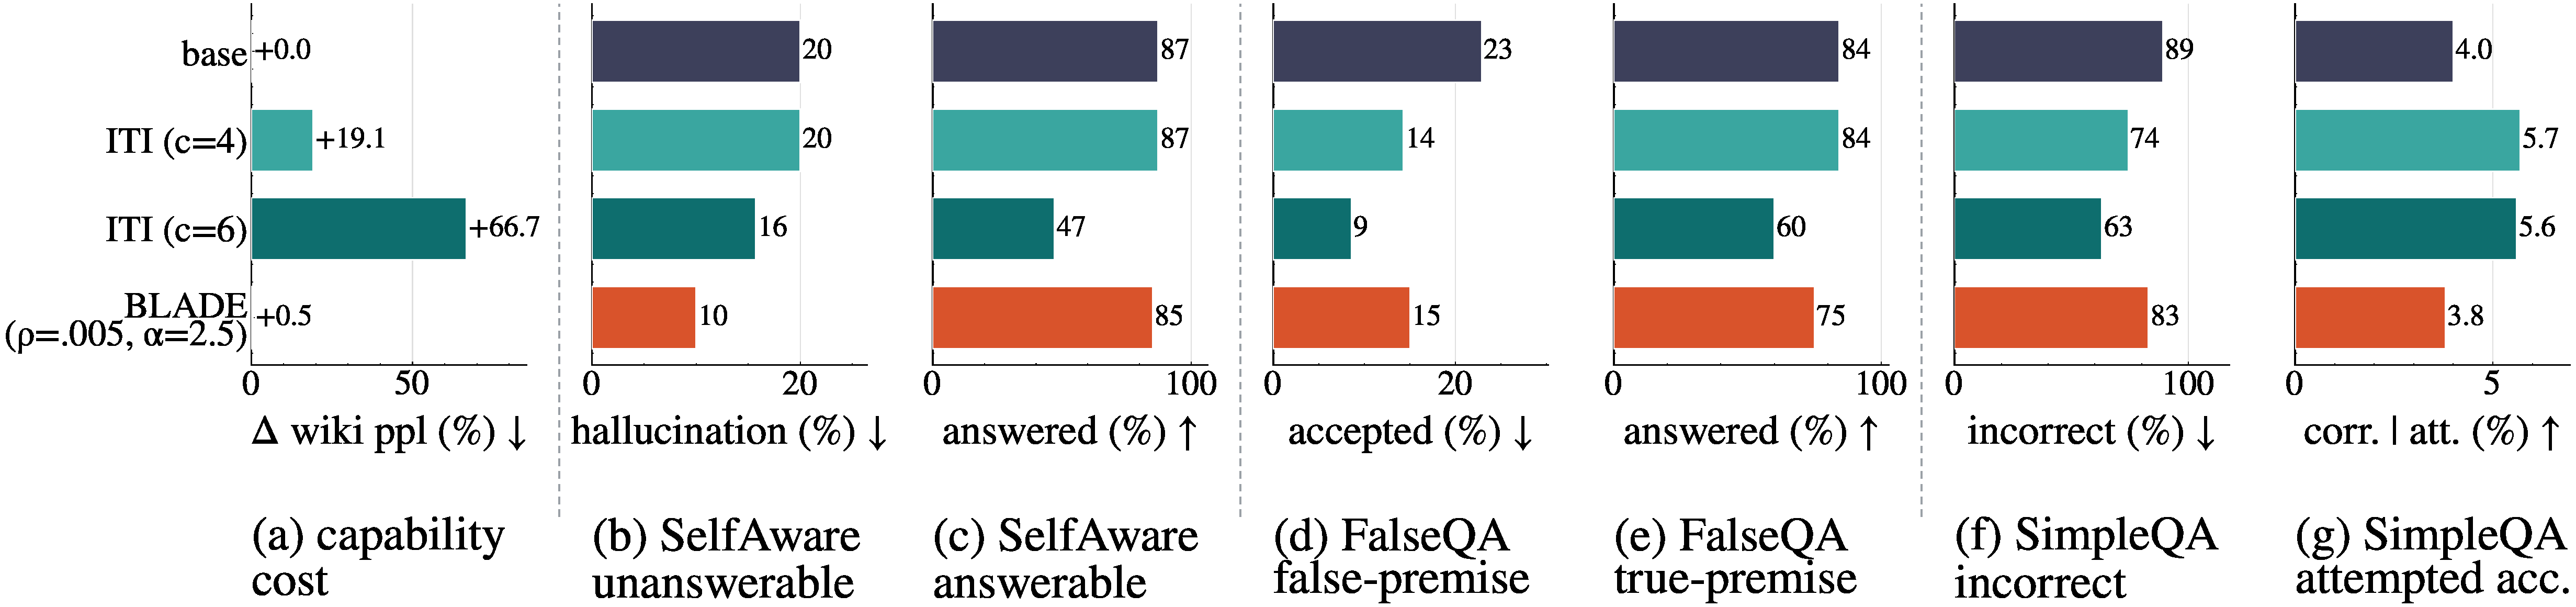
\includegraphics[width=\textwidth]{figures/uncertainty_method_cmp_simpleqa.pdf}
  \caption{%
    \textbf{Controlling closed-book epistemic (un)certainty on Qwen3-8B, across three benchmarks.}
    A single BLADE weight edit ($\rho\!=\!0.005$, $\alpha\!=\!2.5$) vs.\ ITI activation
    steering~\citep{li2023iti} at two strengths ($c\!\in\!\{4,6\}$). SelfAware and FalseQA rates are
    from a blind LLM judge; SimpleQA~\citep{simpleqa} responses are graded correct / incorrect /
    not-attempted against gold answers. Lower is better in (a,\,b,\,d,\,f), higher in (c,\,e,\,g).%
  }
  \label{fig:uncertainty-method-cmp-simpleqa}
\end{figure*}

% ---------------------------------------------------------------------------
% Body text (the "context" for the figure) — paste near the \ref, not in the caption.
% ---------------------------------------------------------------------------
\paragraph{Benchmarks.} We evaluate on three closed-book benchmarks that probe complementary
facets of epistemic (un)certainty. \textbf{SelfAware}~\cite{selfaware} pairs answerable questions
with \emph{unanswerable} ones---open scientific unknowns, under-specified or subjective queries with
no known answer; a calibrated model answers the former and abstains on the latter, so we report the
hallucination rate on the unanswerable half and the answer rate on the answerable half.
\textbf{FalseQA}~\cite{falseqa} pairs questions built on a \emph{false premise} (a presupposition
that is factually wrong) with matched valid-premise questions; here a calibrated model rejects or
corrects the false premise rather than answering as if it held, so we report false-premise acceptance
and true-premise answering. \textbf{SimpleQA}~\cite{simpleqa} is a factuality benchmark of short
fact-seeking questions with a single known gold answer; unlike the first two it is answer-graded, so
each response is bucketed as \emph{correct}, \emph{incorrect} (a confidently wrong answer, i.e.\ a
hallucination), or \emph{not attempted} (an abstention). A model should attempt what it knows and
abstain otherwise; we report the incorrect rate and the attempted accuracy
(correct-given-attempted, $\mathrm{correct}/(\mathrm{correct}+\mathrm{incorrect})$).

Both interventions are fit on the \emph{same} certain/uncertain prompt contrast at the last prompt
token, so the comparison isolates the mechanism---a sparse, static weight edit versus per-head
activation steering---rather than the direction source. We report a single BLADE operating point
($\rho\!=\!0.005$, $\alpha\!=\!2.5$; BLADE-G, thinking-off, layers auto-selected) and ITI at steering
strength $c\!\in\!\{4,6\}$ (in units of per-head projection std; $c$ is ITI's dose, distinct from
BLADE's amplification $\alpha$).

\paragraph{SelfAware and FalseQA.} ITI reduces SelfAware unanswerable hallucination only at a strength
that is catastrophic for capability: it leaves this rate at the base $20\%$ at $c\!=\!4$ and lowers it
to $16\%$ only at $c\!=\!6$, where C4 teacher-forced perplexity rises by $57.3\%$ (panel~a) and
answering on SelfAware answerable questions collapses to $47\%$ (panel~c). BLADE instead lowers
unanswerable hallucination to $10\%$ (panel~b) while holding perplexity essentially flat ($-0.3\%$)
and preserving answering at $85\%$ (base $87\%$). On FalseQA false-premise acceptance (panel~d) BLADE
reaches $15\%$ (base $23\%$), comparable to ITI $c\!=\!4$ ($14\%$, but at $+17.5\%$ perplexity) and
beaten only by the capability-destroying $c\!=\!6$ ($9\%$); BLADE retains most true-premise answering
($75\%$ vs.\ base $84\%$; panel~e).

\paragraph{SimpleQA.} The answer-graded benchmark tells the same story on external factual questions
(panels~f,g; $n\!=\!400$). The base model is badly miscalibrated---it answers almost everything and is
confidently wrong $89\%$ of the time (only $7\%$ abstentions). Both interventions convert confident
errors into abstentions: incorrect drops to $74\%$ (ITI $c\!=\!4$), $63\%$ ($c\!=\!6$), and $72\%$
(BLADE), lifting attempted accuracy from $4.0\%$ to $5.7\%$, $5.6\%$, and $5.6\%$ respectively. BLADE
matches the milder ITI setting while ITI reaches its lowest incorrect rate only at the
capability-destroying $c\!=\!6$. Overall accuracy stays near the floor for all conditions
(Table~\ref{tab:simpleqa}): Qwen3-8B knows the answer to very few SimpleQA questions, so the edit
mainly removes hallucinations rather than adding correct answers, and the attempted-accuracy and
F-score gaps between conditions are correspondingly small.

\begin{table}[t]
\centering
\small
\begin{tabular}{@{}lccccc@{}}
\toprule
Method & Correct & Incorrect & Not att. & Corr.\,$\mid$\,att. & F-score \\
\midrule
base            & 3.8 & 89.0 &  7.2 & 4.0 & 3.9 \\
ITI ($c\!=\!4$) & 4.5 & 74.2 & 21.2 & 5.7 & 5.0 \\
ITI ($c\!=\!6$) & 3.8 & 63.0 & 33.2 & 5.6 & 4.5 \\
BLADE ($\rho\!=\!.005,\alpha\!=\!2.5$) & 4.2 & 71.8 & 24.0 & 5.6 & 4.8 \\
\bottomrule
\end{tabular}
\caption{SimpleQA outcome breakdown (\%; Qwen3-8B, $n\!=\!400$, thinking-off, blind LLM grading).
F-score is the harmonic mean of overall correct and correct-given-attempted~\citep{simpleqa}. Correct
is near the floor for this model, so attempted-accuracy and F differences are small; the clean signal
is the drop in incorrect (hallucination).}
\label{tab:simpleqa}
\end{table}
